\documentclass[11pt,twoside]{article}
\usepackage{geometry}
\usepackage{enumerate}
\usepackage{latexsym,booktabs}
\usepackage{amsmath,amssymb}
\usepackage{graphicx}
\usepackage{hyperref}
\usepackage[singlespacing]{setspace}
\usepackage{calc}
\usepackage{listings}
\usepackage{xcolor}
\usepackage[UKenglish]{datetime}

\definecolor{codegrey}{rgb}{0.5, 0.5, 0.5}
\definecolor{darkpurple}{RGB}{151, 10, 232}
\definecolor{backcolour}{rgb}{0.95, 0.95, 0.92}
\definecolor{forestgreen}{RGB}{5, 155, 50}
\definecolor{codeorange}{RGB}{255, 128, 0}

\lstdefinestyle{mystyle}{
    backgroundcolor=\color{backcolour},   
    commentstyle=\color{forestgreen},
    keywordstyle=\color{blue},
    numberstyle=\tiny\color{codegrey},
    identifierstyle=\color{codeorange},
    stringstyle=\color{darkpurple},
    basicstyle=\ttfamily\footnotesize,
    breakatwhitespace=false,         
    breaklines=true,                 
    captionpos=b,                    
    keepspaces=true,                 
    numbers=left,                    
    numbersep=5pt,                  
    showspaces=false,                
    showstringspaces=false,
    showtabs=false,                  
    tabsize=2
}

\lstset{style = mystyle}

\geometry{a4paper,left=2cm,right=2.0cm, top=2cm, bottom=2.0cm}

\newtheorem{Definition}{Definition}
\newtheorem{Theorem}{Theorem}
\newtheorem{Lemma}{Lemma}
\newtheorem{Corollary}{Corollary}
\newtheorem{Proposition}{Proposition}
\newtheorem{Algorithm}{Algorithm}
\numberwithin{Theorem}{section}
\numberwithin{Definition}{section}
\numberwithin{Lemma}{section}
\numberwithin{Algorithm}{section}
\numberwithin{equation}{section}

\newcommand{\dottedline}[1]{\makebox[#1]{.\dotfill}}

\begin{document}

\pagestyle{empty}

% =============================================================================
% Title page
% =============================================================================
\begin{titlepage}
\vspace*{.5em}
\center
\textbf{\Large{The School of Mathematics}} \\
\vspace*{1em}
\begin{figure}[!h]
\centering

\includegraphics[width=180pt]{CentredLogoCMYK.jpg}
\end{figure}
\vspace{2em}
\textbf{\Huge{My Incredible Thesis}}\\[2em]
\textbf{\LARGE{by}}\\
\vspace{2em}
\textbf{\LARGE{Robin Lin}}\\
\vspace{6.5em}
\Large{Dissertation Presented for the Degree of\\
MSc in Statistics with Data Science}\\
\vspace{6.5em}
\Large{\today}\\
\vspace{3em}
\Large{Supervised by\\Dr Nicole Augustin and Dr Michael Allerhand}
\vfill
\end{titlepage}

\cleardoublepage

% =============================================================================
% Executive summary, acknowledgments, and own work declaration
% =============================================================================
\begin{center}
\Large{Executive Summary}
\end{center}

Here comes your executive summary ...

\clearpage

\begin{center}
\Large{Acknowledgments}
\end{center}

Here come your acknowledgments ...

\clearpage

\begin{center}
\Large{University of Edinburgh – Own Work Declaration}
\end{center}


This sheet must be filled in, signed and dated - your work will not be marked unless this is done.
\vspace{1cm}

Name: \dottedline{8cm}

Matriculation Number: \dottedline{6cm}

Title of work: \dottedline{8cm}

\vspace{1cm}

I confirm that all this work is my own except where indicated, and that I have:
\begin{itemize}
\item	Clearly referenced/listed all sources as appropriate	 				
\item	Referenced and put in inverted commas all quoted text (from books, web, etc)	
\item	Given the sources of all pictures, data etc. that are not my own				
\item	Not made any use of the report(s) or essay(s) of any other student(s) either past 	
or present	
\item	Not sought or used the help of any external professional academic agencies for the work
\item	Acknowledged in appropriate places any help that I have received from others	(e.g. fellow students, technicians, statisticians, external sources)
\item	Complied with any other plagiarism criteria specified in the Course handbook
\end{itemize}

I understand that any false claim for this work will be penalised in accordance with
the University regulations	(\url{https://teaching.maths.ed.ac.uk/main/msc-students/msc-programmes/statistics/data-science/assessment/academic-misconduct}).								

\vspace{1cm}

Signature \dottedline{8cm}

\vspace{5mm}

Date \dottedline{8cm}


\clearpage



% =============================================================================
% Table of contents, tables, and pictures (if applicable)
% =============================================================================
\pagestyle{plain}
\setcounter{page}{1}
\pagenumbering{Roman}

\tableofcontents
\clearpage
\listoftables
\listoffigures
\cleardoublepage

\pagenumbering{arabic}
\setcounter{page}{1}

\nocite{*}
\bibliographystyle{abbrv}
\clearpage

\section{Introduction}
\label{sec:intro}
\subsection{Overview}
\href{https://www.simplybusiness.co.uk/}{\textit{Simply Business}} is one of the largest providers of business and landlord insurance in the UK. Such a provider works on determining premiums that customers need to pay for their property insurance. When the premiums are being estimated, various risk factors are taken into account, including the types and sizes of properties, the number of rooms, and the characteristics of the constructions, etc. Among all risk factors, the types of properties are vitally important for insurance companies. A possible reason for that could be the variations in shapes and materials in the construction processes of properties. Such differences could have an impact on whether they are easy to get damaged in various situations. For instance, the ability of a round-shaped facade to avoid being knocked down by strong wind is often higher than that of a flat one. Also, brick houses are not as easily burnt by fire as wood ones. Such information is used by insurance providers to adjust the policies to their customers accordingly.

\subsection{Data Description and Project Objectives}
In this project, the street view images and datasets to be used are provided by \href{https://www.simplybusiness.co.uk/}{\textit{Simply Business}}. Multiple images are extracted from the latest Google street view data, with a unique identity number attached to each of them. Multiple datasets are extracted from \href{https://www.rightmove.co.uk/}{\textit{Rightmove} website}, clearly showing the necessary information of the properties as follows.

\begin{itemize}
    \item Addresses
\item Property Types
\item Numbers of Bedrooms
\item Web Links
\item Location Coordinates
\item Identity Numbers
\end{itemize}






For the images, their property types could be extracted from one of the given datasets by providing the identity numbers attached to them, allowing the types of properties to be linked with the images. The main objectives of this project are to estimate the types of properties by constructing different models given the images from Google street view, and to select a model with the best accuracy, so that the types of properties could be detected automatically. It is worth estimating the types of properties, in that some customers might have failed to reveal the information regarding their properties, or they might have provided the wrong information. Since images from Google street view data are novel, such intuitive and figurative information could be able to reveal the housing status of a customer authentically.

\subsection{Characteristics of the Properties and Street View Images}
As mentioned above, the datasets clearly show the information of the properties. These datasets also share exactly the same attributes, making it easy for us to merge the entries from different datasets into a new data frame. In the new data frame, there are $37,402$ entries in total, and no missing values are found for the property types. However, not every property has an attached street view image. In this case, only the properties with street view images attached would be taken into account in the models. The number of such kind of properties is $35,744$. However, this does not necessarily mean that the number of unique street view images is $35,744$, and in fact a large number of duplicate images are spotted. Although the duplicate images have different identity numbers attached to them, they share exactly the same latitudes and longitudes. In the future models, overfitting issue might occur if a large amount of duplicate images are taken into account in the models, since there would be more noise affecting the performances of the models. In view of this, such duplicate images should be discarded, and there are $15,484$ unique images. In the new data frame, the entries corresponding to the duplicate images should also be removed accordingly. Those entries are the ones with the same values of latitudes and longitudes. The number of unique properties is hence $15,484$.

The unique properties are scattered on the UK map as follows in Figure \ref{fig:locations}. 


\begin{figure}[h]
\centering
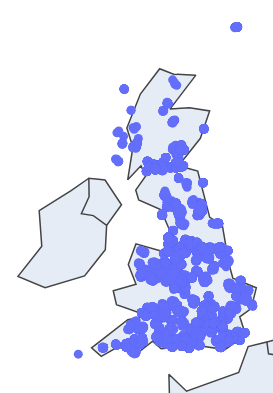
\includegraphics[scale = 1]{1/MSc_LaTeX_SwDS/MSc_LaTeX_SwDS/Plots/Locations.png}
\caption{Locations of the Properties}
\label{fig:locations}
\end{figure}

At first glance, it could be observed that the properties are selected from Great Britain and some other small isles of Britain. By having a closer look into it, it could be observed that the properties are mostly extracted from the middle and south of England, north of Wales, Glasgow, and Edinburgh. There are also a few properties located in the north of England, as well as in the north of Scotland.

There are $4$ types of properties considered in this project, which are detached, flat, semi-detached, and terraced. However, there are $5$ classes in the variable “property types”, and the other class not specified above is the “unknown” one. When street view images are labelled as “unknown”, there could be at least one possible type of property, or it could be the case where none of the $4$ types best describe the characteristics of the properties in the street view images. The percentages of the $5$ classes are shown as follows in Figure \ref{fig:pie}. 

\begin{figure}[h]
\centering
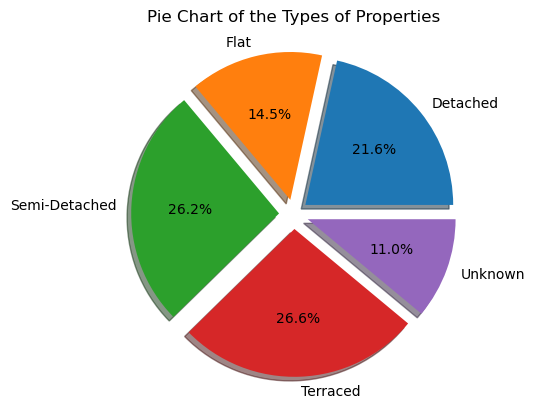
\includegraphics[scale = .7]{1/MSc_LaTeX_SwDS/MSc_LaTeX_SwDS/Plots/Pie.png}
\caption{Pie Chart of the Types of Properties}
\label{fig:pie}
\end{figure}

From the pie chart, it could be observed that the classes are not evenly divided, indicating that the data set is imbalanced. An imbalanced dataset could be harmful in the models. When a model is being trained, it could probably keep predicting the classes that have higher proportions, in order that a higher accuracy in the training sets could be achieved. However, when it comes to validating and testing the model, the performances of classes with lower proportions might not be decent enough. In addition, classes with lower proportions might not be able to learn as much as the other classes do, leading to lower accuracy in model prediction. In view of this, some perturbations are to be made in the loss function, which would be discussed in later sections.

As mentioned above, there are $5$ classes in the variable “property types”, and one of the classes is “unknown”. It is crucial to discuss whether to have the images labelled as “unknown” kept as they are, or to have them discarded, as this might have an impact on the performances of the models. There is no harm in looking at some example images first. As mentioned above, it could be the case where none of the 4 types best describes the characteristics of the properties. As shown in Figure \ref{fig:unknown_green_road}, if images mostly contain objects that are in green, such as trees or forests, or when they contain a road without a house, the models might learn them as a pattern, and classify property types correctly as “unknown”. However, such a case only occurs in a very small portion of images. 

\begin{figure}[h]
\centering
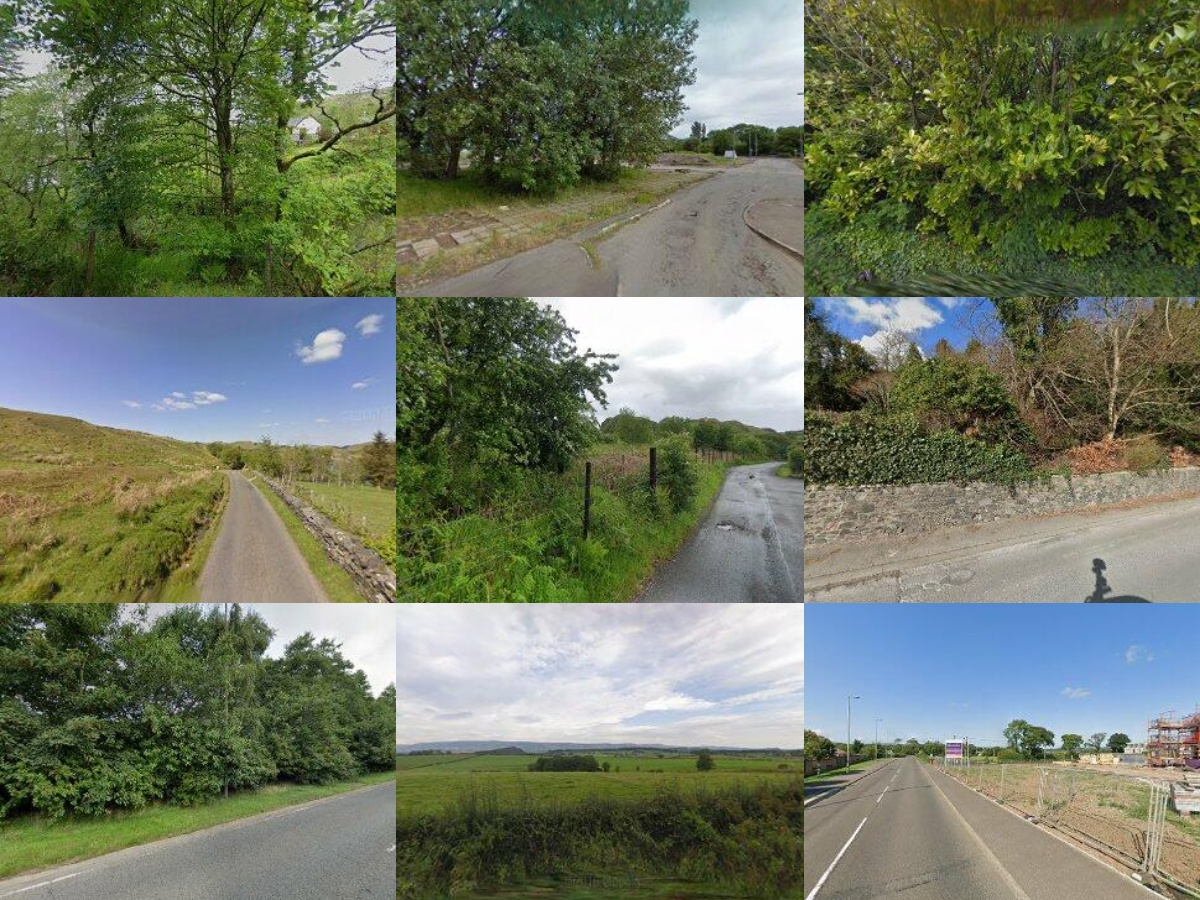
\includegraphics[scale = .2]{1/MSc_LaTeX_SwDS/MSc_LaTeX_SwDS/Labelled Unknown/no_houses.jpg}
\caption{Examples of Properties Labelled “Unknown” without a House}
\label{fig:unknown_green_road}
\end{figure}

In general, there are houses in most images labelled “unknown”, so there is a greater chance that at least one possible type of property is in the images, as shown in Figure \ref{fig:unknown_houses}. 

\begin{figure}[h]
\centering
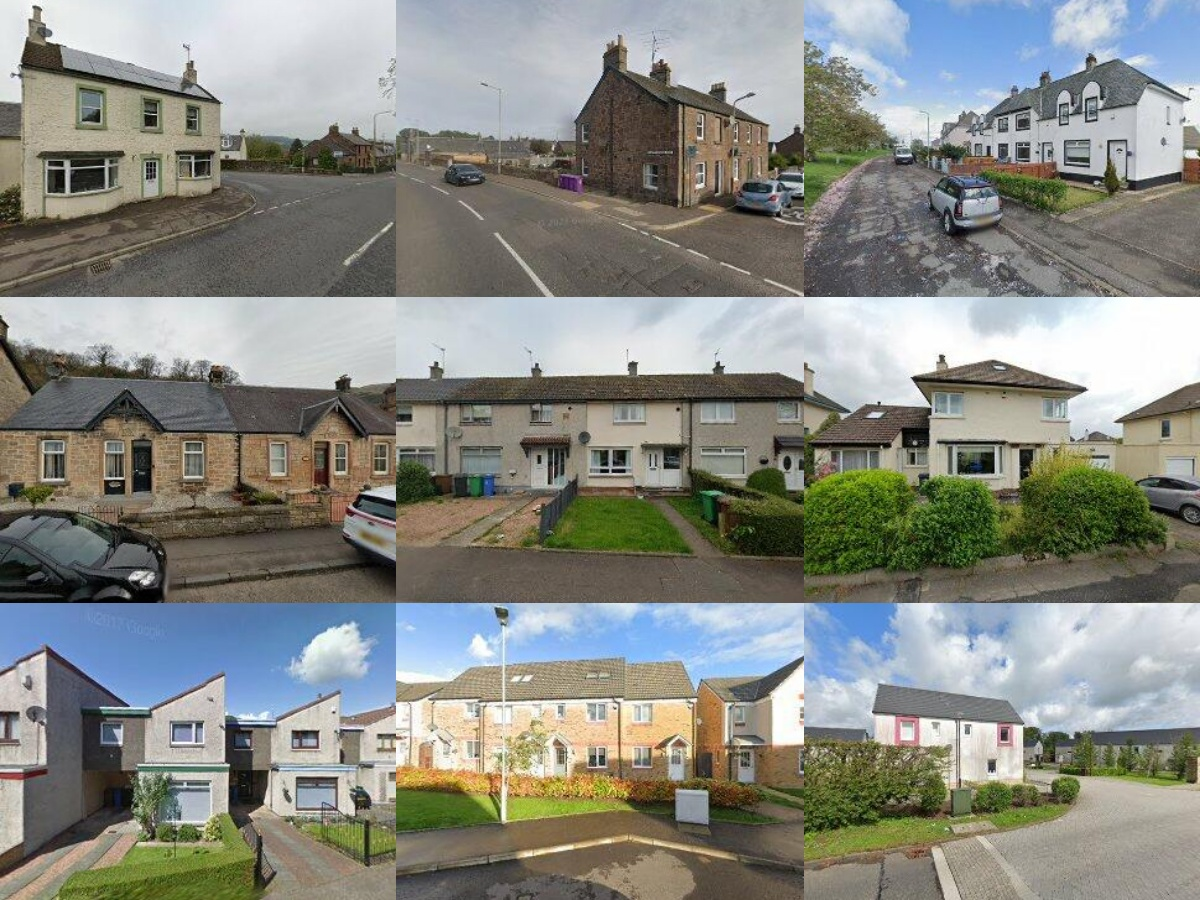
\includegraphics[scale = .2]{1/MSc_LaTeX_SwDS/MSc_LaTeX_SwDS/Labelled Unknown/apparent_houses.jpg}
\caption{Examples of Properties Labelled “Unknown” with Houses}
\label{fig:unknown_houses}
\end{figure}

When models are being trained, the contours of the houses might be captured and sketched by them. After the models are trained, they should be validated and tested, and the contours are key information in classifying the types of houses. This could lead to a situation where the models classify objects in the images as one of the $4$ types of properties, instead of classifying them as “unknown”, indicating that the accuracy of validation and testing would be very low. Moreover, “unknown” is not a type of property being widely acknowledged by people, and hence it does not make any sense to classify the images as this type. Therefore, the images labelled “unknown” are ignored, along with their corresponding entries in the new data frame. The number of images to be considered should hence be $13,775$.

\subsection{A Literature Review on Image Classification Models}
A brief review of the literature is provided, presenting the models applied in classification of images, especially Google street view images, in recent years. In 2016, the authors of \cite{ahmed2016house} extracted visual and textural features, and fed them into a multi-layer perceptron (MLP) model and a support vector regression (SVR) model. They concluded that their MLP model performed better than their SVR model. In 2017, the authors of \cite{law2017application} applied the convolutional neural network (CNN) model to classify the frontages of street view images in Greater London and found decent results in their model. In 2018, the authors of \cite{kang2018building} applied VGG16, a special kind of CNN model, to classify the facade structures from Google street view images, and achieved high accuracy. In 2019, the authors of \cite{law2019take} applied CNN and Generalised Additive Model (GAM) to the Google street view images from different angles in predicting house prices in London, and found promising results. In 2020, the authors of \cite{avelar2020superpixel} adopted Graph Neural Network (GNN) models in classifying superpixel images, which was an unprecedented experiment, and they successfully classified panoramas. Finally, in 2021, the authors of \cite{maniat2021deep} also adopted VGG16 to detect visual cracks in pavement images, which were extracted from Google street view, and managed to classify those images into different categories of cracks.

From the above literature, it could be observed that people tend to use CNN, especially the newly invented VGG16, to classify street view images. There are cases where people use the traditional MLP and SVR models. In this project, more than $10,000$ images are to be trained, and it does not seem time-efficient to train such a large amount of images using SVR models. Moreover, VGG16 model looks too fancy to be implemented, since such kind of model has a complex structure, and overfitting issue might occur more easily when such a model is adopted. Therefore, simple MLP and CNN models are adopted in this paper.

\section{Preliminary Settings}
\label{sec:prelim}
\subsection{Downsizing Images}
The street view images are reformatted into matrices with $3$ axes. The first axis describes the height of an image, and there are $320$ pixels along this axis. The second one describes the width of an image, and there are also $320$ pixels along this axis. The third one describes the number of primary colours. After reformatting, $307, 200$ pixel values are generated for each image, and such values are integers ranging from $0$ to $255$. However, there could be an issue of memory if a large amount of features are taken into account in constructing models. A possible way to avoid it could be applying dimensionality reduction techniques, including principle component analysis (PCA), and factor analysis. However, chances are that crucial information might be lost when applying such techniques. For instance, contours of the houses might be necessary for image classification, and if some of those key pixels are missing, models might provide ridiculous results, such as classifying a flat as a terraced house. In view of this, dimensionality reduction techniques would not be the best option. Another possible way could be extracting features by applying algorithms like autoencoder, or diffusion map, etc. However, none of these algorithms seem time-efficient in dealing with such a large scale of features in the images. The fastest, and perhaps the most straightforward method is resizing those images to a lower resolution. It should be very fast, since it is just about merging, and averaging neighbouring pixels. It should also preserve the key information in the images, since downsizing them would preserve the information of the contours of houses, which might be crucial in modelling. In this project, the heights and widths of the images are downsized to $64$ pixels. The main advantages of doing so are that training a model would not be extremely time consuming, and that key information, such as the contours of houses, would be preserved.

\subsection{One Hot Encoding}
For the categorical outcome variable, one hot encoding is applied to convert it into a numerical form. Such an encoding method preserves norminality of the variable, ensuring that the models learn patterns of the outcome variable.

\subsection{Train-Validation-Test Split}
The models adopted in this paper are neural network models. In order to avoid overfitting, it is necessary to split a dataset into different groups. In this project, the dataset is split into non-overlapping training, validation, and test sets by randomly selecting an integer-valued seed. Among the $3$ sets, there are $70\%$ of the data in the training set, $20\%$ in the validation set, and the rest $10\%$ in the testing set.

\section{Modelling}


\section{Results}
\label{sec:results}
I this section, I explain what did I discover.

Now it's getting very technical \ldots{} I will cite \cite{shiina,groewe2001}. I will also show my incredible $\alpha$, $\beta$ and $\gamma$ mathematics and do some other fancy stuff.

\subsection{Formulae}

For example look at this
\begin{equation}\label{eqn:aProblem}
\min{}\sum_{s\in\mathcal{S}}Pr_{s}\left[\sum_{t=1}^{T}\left(
\sum_{g\in\mathcal{G}}\left(\alpha_{gts}C_{g}^{0}+
p_{gts}C_{g}^{1}+\left(p_{gts}\right)^{2}C_{g}^{2}\right)
+\sum_{g\in\mathcal{C}}\gamma_{gts}C_{g}^{s}\right)\right],
\end{equation}
and you will see that it has a little number on the side so that I can refer to it as equation (\ref{eqn:aProblem}). Now if I do this
\begin{eqnarray}
\sum_{i=1}^{n}k_{i}&=&20\label{eqn:one}\\
\sum_{j=20}^{m}\delta_{i}&\geq{}&\eta{}\notag
\end{eqnarray}
I can align two formulae and control which one has a number on the side. It is (\ref{eqn:one}). I can also do something like this
\begin{displaymath}
Y_{l}=\left[\begin{array}{cc}
             \left(y_{s}+i\frac{b_{c}}{2}\right)\frac{1}{\tau{}^{2}} &
             -y_{s}\frac{1}{\tau{}e^{-i\theta^{s}}}\\
             -y_{s}\frac{1}{\tau{}e^{i\theta^{s}}} &
             y_{s}+i\frac{b_{c}}{2}
             \end{array}\right],
\end{displaymath}
and it won't have a number on the side. Now if I have to do some huge mathematics I'd better structure it a little and include linebreaks etc. so that it fits on one page.
\begin{eqnarray}\label{eqn:horrible}
p_{l}^{f}&=&G_{l11}\left(2v_{F(l)}\bar{v}_{F(l)}-\bar{v}_{F(l)}^{2}\right)\\
&+&
\bar{v}_{F(l)}\bar{v}_{T(l)}
\left[
B_{l12}\sin{}(\bar{\delta{}}_{F(l)}-\bar{\delta{}}_{T(l)})
+G_{l12}\cos{}(\bar{\delta{}}_{F(l)}-\bar{\delta{}}_{T(l)})
\right]\notag\\
&+&
\left[\begin{array}{r}
      \bar{v}_{T(l)}
      \left[
      B_{l12}\sin{}(\bar{\delta{}}_{F(l)}-\bar{\delta{}}_{T(l)})
      +G_{l12}\cos{}(\bar{\delta{}}_{F(l)}-\bar{\delta{}}_{T(l)})
      \right]\\
      \bar{v}_{F(l)}
      \left[
      B_{l12}\sin{}(\bar{\delta{}}_{F(l)}-\bar{\delta{}}_{T(l)})
      +G_{l12}\cos{}(\bar{\delta{}}_{F(l)}-\bar{\delta{}}_{T(l)})
      \right]\\
      \bar{v}_{F(l)}\bar{v}_{T(l)}
      \left[
      B_{l12}\cos{}(\bar{\delta{}}_{F(l)}-\bar{\delta{}}_{T(l)})
      -G_{l12}\sin{}(\bar{\delta{}}_{F(l)}-\bar{\delta{}}_{T(l)})
      \right]\\
      \bar{v}_{F(l)}\bar{v}_{T(l)}
      \left[
      -B_{l12}\cos{}(\bar{\delta{}}_{F(l)}-\bar{\delta{}}_{T(l)})
      +G_{l12}\sin{}(\bar{\delta{}}_{F(l)}-\bar{\delta{}}_{T(l)})
      \right]\\
      \end{array}\right]
\cdot{}
\left[\begin{array}{c}
      v_{F(l)}-\bar{v}_{F(l)}\\
      v_{T(l)}-\bar{v}_{T(l)}\\
      \delta_{F(l)}-\bar{\delta{}}_{F(l)}\\
      \delta_{T(l)}-\bar{\delta{}}_{T(l)}
      \end{array}\right],\notag
\end{eqnarray}
This is a lot of fun!
\clearpage

\subsection{Important Things}
Finally we should have a nice picture like this one. However, I won't forget that figures and table are environments which float around in my document. So LaTeX will place them wherever it thinks they fit well with the surrounding text. I can try to change that with a float specifier, e.g. [!ht].
%This is a comment. The Compiler ignores it. It is here to remind me that, if I use a .jpeg or .png picture file as below I will need to compile 
classes are shown as follows in Figure 2.
Figure 2: Pie Chart of the Types of Properties
From the pie chart, it could be observed that the classes are not evenly divided, indicating that
the data set is imbalanced. An imbalanced dataset could be harmful in the models. When a model is being trained, it could probably keep predicting the classes that have higher proportions, in order that
a higher accuracy in the training sets could be achieved. However, when it comes to validating and
testing the model, the performances of classes with lower proportions might not be decent enough. In
addition, classes with lower proportions might not be able to learn as much as the other classes do,
leading to lower accuracy in model prediction. In view of this, some perturbations are to be made in
the loss function, which would be discussed in later sections.
As mentioned above, there are 5 classes in the variable “property types”, and one of the classes is
“unknown”. It is crucial to discuss whether to have the images labelled as “unknown” kept as they
are, or to have them discarded, as this might have an impact on the performances of the models.
There is no harm in looking at some example images first. As mentioned above, it could be the case
where none of the 4 types best describes the characteristics of the properties. As shown in Figure 3, if
images mostly contain objects that are in green, such as trees or forests, or when they contain a road
without a house, the models might learn them as a pattern, and classify property types correctly as
“unknown”. However, such a case only occurs in a very small portion of images.
Figure 3: Examples of Properties Labelled “Unknown” without a House
In general, there are houses in most images labelled “unknown”, so there is a greater chance that
at least one possible type of property is in the images, as shown in Figure 4.
Figure 4: Examples of Properties Labelled “Unknown” with Houses
When models are being trained, the contours of the houses might be captured and sketched by
them. After the models are trained, they should be validated and tested, and the contours are key
information in classifying the types of houses. This could lead to a situation where the models classify
objects in the images as one of the 4 types of properties, instead of classifying them as “unknown”,
3


the document with the pdflatex compiler.

Now I want to use one of my own environments. I want to define something.
\begin{Definition}
 I define
$$
\Gamma_{\eta}:=\sum_{i=1}^{n}\sum_{j=i}^{n}\xi{}(i,j)
$$
\end{Definition}
I definitely need some good tables, so I do this.
\begin{table}[!ht]
\centering
\begin{tabular}{|ll|rrrr|}
\hline
Case&Generators&Therm. Units&Lines&Peak load: [MW]&[MVar]\\
\hline\hline
6 bus&3 at 3 buses&2&11&210&210\\
9 bus&3 at 3 buses&3&9&315&115\\
24 bus&33 at 11 buses&26&38&2850&580\\
30 bus&6 at 6 buses&5&41&189.2&107.2\\
39 bus&10 at 10 buses&7&46&6254.2&1387.1\\
57 bus&7 at 7 buses&7&80&1250.8&336.4\\
\hline
\end{tabular}
\caption{Something that doesn't make sense.}
\label{tab:things}
\end{table}
I should really refer to Table \ref{tab:things}.

\subsection{And now something else}

\noindent
Let:
\begin{eqnarray*}
\Omega_0 & = & \{(x,y,z,f): \text{ satisfying } (9)-(19)\}, \\
\Omega_1 & = & \{(x,y,z,f): \text{ satisfying } (9),(11)-(20)\}, \\
\overline{\Omega}_0 & = & \{\textbf{0}\leq (x,y,z,f) \leq \textbf{1}: \text{ satisfying } (9)-(18)\}, \\
\overline{\Omega}_1 & = & \{\textbf{0}\leq (x,y,z,f) \leq \textbf{1}: \text{ satisfying } (9),(11)-(18),(20)\} \,.
\end{eqnarray*}
%
where $\textbf{0}$ and $\textbf{1}$ are vectors of appropriate dimensions with 0's and 1's, respectively.
Next we see that both $\Omega_0$ and $\Omega_1$ give equivalent formulations for the A-MSSP. In particular, the following statements hold:

\begin{Proposition}
$\Omega_0 \subseteq \Omega_1$.
\end{Proposition}

\noindent
\textbf{Proof.}
Let us suppose there exists $(x,y,z,f) \in \Omega_1$ such that $(x,y,z,f) \notin \Omega_0$.
Then, there exist indices $i \in I$ and $t \in \{0,\ldots,|T|-s_i\} $ with $x_i^t > \displaystyle 0.5\,\left( \sum_{h=1}^{s_i} x_i^{t+h} +1\right)$.
By definition, $x_i^t = 1$ and $x_i^{t+h} = 0$ for all $h \in \{1,\dots,s_i\}$. By~(11) and (12), $\displaystyle \sum_{h=1}^{s_i} f_i^{th}=1$, so $f_i^{th'}=1$ for some $h' \in \{1,\dots,s_i\}$.
But then,
\[ 0 \:=\: x_i^{t+h'} \:=\: \sum_{h=\max \{1, t+h'-(|T|-s_i)\}}^{\min\{s_i,t+h'\}} f_i^{t+h'-h,h} \:\ge\: f_i^{th'} \:=\: 1 \,,
\]
as $h' \in [\max \{1, t+h'-(|T|-s_i)\}, \min\{s_i,t+h'\}]$.
\hfill $\square$
\bigskip

\noindent
This immediately gives us
\begin{Corollary}
AS is a valid formulation for the A-MSSP.
\end{Corollary}

\noindent
Next we compare the Linear Programming (LP) relaxations of the two formulations.

\begin{Proposition}
$\overline{\Omega}_1 \subseteq  \overline{\Omega}_0 $.
\end{Proposition}

\noindent
\textbf{Proof.}
Homework
\hfill $\square$
\cleardoublepage


\section{Conclusions}
I have no idea how to conclude, so I don't write much. But the stuff that follows is important.
\clearpage

%the entries have to be in the file literature.bib
\bibliography{literature}
\clearpage

\appendix
\section*{Appendices}
\addcontentsline{toc}{section}{Appendices}

\section{An Appendix}
\label{app:one}

Some stuff.

\begin{lstlisting}[language = Python]
require(survival)
require(survminer)

# Kaplan-Meier plot by aetiology
km.aet <- survfit(Surv(TimeB, Status == 1) ~ Princ.aetio.simp,
data = screen.hcc.agg)

ggsurvplot(km.aet,
censor = F,
size = 0.5,
ggtheme = theme_gray(),
font.main = 9, font.x = 9, font.y = 9, font.legend = 8,
legend = "right",
xlab = "Time (days)") +
scale_color_hue(labels = c("ALD", "AID", "HepB", "HepC",
"NAFLD", "Other")) +
guides(color = guide_legend(title = "Princ. aetiology"))

# Log-rank test
survdiff(Surv(TimeB, Status == 1) ~ Princ.aetio.simp,
data = screen.hcc.agg)

\end{lstlisting}

\clearpage

\section{Another Appendix}
\label{app:two}

Some other stuff.

\end{document}
